\section{File System}
\label{section: file system}

	% Section overview.
	The file system is certainly the largest and most complex subsystem
	in Nanvix. It extends the hardware abstraction layer and exports
	through the file abstraction a uniform interface for dealing with
	bare resources. In this section we take a closer look in this
	subsystem. We first present the buffer cache, an internal module
	that speedups the performance of the file system, and then we move
	our discussion to the file system's layout, structure and internals.

	\subsection{The Buffer Cache Module}
	\label{subsection: the buffer cache module}

	\begin{figure}[t]
		\centering
		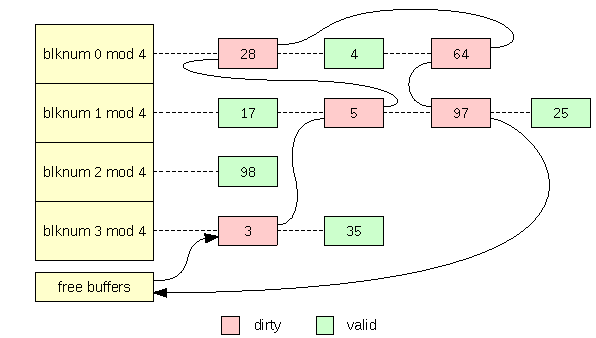
\includegraphics[scale=1]{img/buffer-cache}
		\caption{Buffer cache.}
		\label{figure: buffer cache}
	\end{figure}

	% Buffer cache module overview.
	Most requests that arrive at the file system involve disk I/O
	operations. If, in order to handle each of them, the file system
	would have to issue an I/O operation, the system's performance would
	be awful. Therefore, to get around this problem, the file system
	buffers disk blocks in memory and also maintains a cache of most
	frequently used buffers there, as shown in Figure \ref{figure:
	buffer cache}. In this cache, all buffers are hashed in a table
	according to the number of the disk block that they currently hold,
	and buffers that are not in use are linked in a list structure. This
	way, any buffer can be quickly retrieved through the hash table, and
	the kernel can easily get a free buffer from the list, whenever it
	needs one.

	% Buffer cache routines #1.
	The buffer cache module exports a set of routines to other
	subsystems to enable them manipulate buffers. To read a buffer from
	the cache, the \texttt{bread()} routine is provided. Internally,
	this routine searches the buffer cache for a specific block and
	returns a pointer to it. If the requested block is not in the buffer
	cache, its contents are read from disk to some buffer. What buffer
	will be be used to handle the request may come from two different
	sources. If the list of free buffers is not empty, the kernel claims
	a buffer from there and uses it in the operation. However, if this
	list is empty, a buffer from the cache is evicted to disk, according
	to a least-recently used policy, and then it is used to handle the
	\texttt{bread()} request.

	% Buffer cache routines #2.
	After retrieving a block buffer from the buffer cache, subsystems
	may freely read/write data from/to the buffer. Nevertheless, it is
	important to point out that buffers are indeed shared resources, and
	thus to consistently operate these structures subsystems should
	carefully use locking mechanisms. To handle this situation, the
	buffer  buffer cache module provides the \texttt{blklock()} and
	\texttt{blkunlock()} routines, to enable buffers to be locked and
	unlocked respectively. Finally, when a subsystem is done with a
	buffer, it calls \texttt{bwrite()} to release it. If no more
	processes are using that buffer, its contents are flushed to the
	underlying device and then the buffer is marked as ``not used''.

	% Asynchronous read, delayed write.
	As a final remark, it is worthy to note two techniques that are
	supported by the buffer cache to further improve the system's
	performance. The first technique, namely delayed write, is outlined
	in Figure \ref{figure: buffer cache} and works as follows. As we
	detailed before, not-used buffers are linked in a list of free
	buffers, so that the kernel can easily get a buffer whenever it
	needs one. Note, however, that buffers that are not being used also
	appear in the hashing structure. The buffer cache does so in the
	hope that those buffers will soon be need, and thus tries to
	postpone writing as much as possible. The second technique, known as
	asynchronous read, improves the overall system usage by having read
	operations to take place asynchronously, rather than synchronously
	to the process' execution flow. To enable this, the buffer cache
	handles a read operation as it would normally do, however, instead
	of scheduling a synchronous read operation in the disk driver, it
	schedules an asynchronous one and immediately returns. The process
	may then go compute something else, and when the content of the
	buffer gets valid, it is notified about this event.

	\subsection{File System Layout and Structure}
	\label{subsection: file system layout and structure}

	\begin{figure}
		\centering
		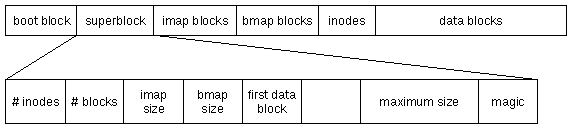
\includegraphics[scale=1.05]{img/file-system-layout}
		\caption{File system layout.}
		\label{figure: file system layout}
	\end{figure}

	% File system overview.
	Nanvix adopts an hierarchical file system based on inodes, which
	heavily resembles the original System V file system reported in
	\cite{Bach:86}. Indeed, the Nanvix file system has been
	intentionally designed to be somewhat compatible with the Minix 1
	file system, so that existing user-level utilities specifically
	designed to manipulate this file system could be used in early
	development phases\footnote{Since version 1.1 Nanvix is shipped with
	its own utilities for sake of portability.}. The Nanvix file system
	is outlined in Figure \ref{figure: file system layout} and detailed
	next.

	% File system layout.
	The Nanvix file system works with 1 KB blocks and it is divided in
	two major zones, one that stores meta information about the file
	system itself and another one that actually holds user data. The
	very first block in the meta information zone stores the bootloader,
	a very small and special program that setups all machine dependent
	features and actually loads the kernel. Following the boot block, is
	the superblock, the place where information concerning the file
	system's peculiarities are kept. For instance, it holds how many
	data blocks and inodes the file system has, what is the maximum size
	for a file size and what is the file system version. After this
	block, there are the inode-map (imap) and block-map (bmpap) blocks,
	which are used for managing disk space; and the inode blocks, which
	store all inodes of the file system. Finally, data blocks hold user
	data, and are linked to the file system hierarchy through the inode
	structure.

	% Inode structure.
	In turn, an inode is a low-level abstraction of a file. It stores
	information concerning the file's type, owner, access permissions,
	current size, time of last modification, and blocks pointers, as it
	is shown in Figure \ref{figure: inode structure}. Data blocks are
	assigned using an hierarchical addressing scheme, where the first
	seven data blocks are directly addressed, and next ones are
	addressed via either double or triple indirections. The way that
	blocks pointers are actually used depend on the type of the file
	itself. If it is a regular file, then blocks pointers point to data
	blocks filled with user data. If the file is a directory, however,
	block pointers point to data blocks that store directory entries.
	Finally, if the file is a special file, the block pointers hold the
	minor and major numbers of the referred device.

	\begin{figure}
		\centering
		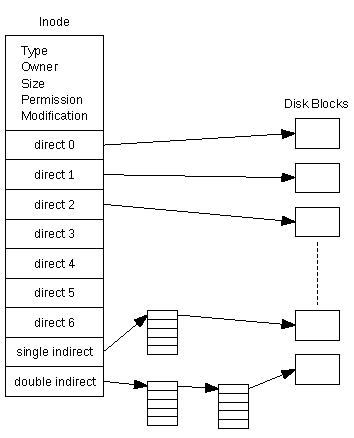
\includegraphics[scale=1.1]{img/inode-structure}
		\caption{Inode Structure.}
		\label{figure: inode structure}
	\end{figure}

	\subsection{File System Internals}
	\label{subsection: file system internals}

		% File system internals section overview.
		So far we have explored the buffer cache module and the file
		system layout. In this section, however, we turn our attentions
		to the file system internals. We first discuss how disk space is
		actually managed, then we introduce the interface that is
		exported for dealing with inodes, and finally we detail some
		kernel routines for manipulating files.

		% Disk space management.
		The file system manages disk space with the help of the
		\texttt{bmap} and \texttt{imap} blocks (see Section
		\ref{subsection: file system layout and structure}). These are
		indeed bitmaps that point out which data blocks and inodes are
		currently in use in the file system, respectively. Whenever an
		inode or a data block needs to bee allocated, the correspondent
		bitmap is sequentially searched for an inode/data block that is
		available. To speedup the search, the kernel maintains these
		bitmaps in memory and from time to time it writes them back to
		disk. Additionally, the kernel keeps track of the last allocated
		bit in each bitmap and uses bitwise operations to perform the
		search. This way, the first free bit in a bitmap can be find
		slightly fast, if the disk is not heavily fragmented, and search
		time is decreased by a factor of $n$, where $n$ is the width in
		bits of the largest machine register. To allocate and free data
		blocks the kernel exports two routines, namely
		\texttt{block\_alloc()} and \texttt{block\_free()}; and
		conversely does the same for inodes, through the
		\texttt{inode\_alloc()} and \texttt{inode\_free()} routines.

		% Inode interface #1.
		Inodes are low-level abstractions for files, and are used to
		model regular files, directories and devices. The most relevant
		routines for manipulating such structures are presented in Table
		\ref{table: inodes interface} and briefly discussed next.
		Ultimately, inodes are stored in disk, so that changes in the
		file system can persist over time. However, to further improve
		the file system's performance, the kernel caches in memory the
		most recently used inodes, in a similar way as it does with disk
		blocks (see Section \ref{figure: buffer cache}). To get an inode
		from the inode cache, the file system exports the
		\texttt{inode\_get()} routine. If the requested inode is in the
		cache, a pointer to it is immediately returned. However, if the
		inode is not in the cache, the kernel reads it from the disk,
		first evicting not-in-use inodes using a least recently used
		strategy if needed. Conversely, the \texttt{inode\_put()}
		routine is provided to release an in-memory inode, making
		available the correspondent slot in the inode cache. Finally, to
		sync the in-memory inodes with in-disk inodes, the file system
		provides the \texttt{inode\_sync()} routine. This call iterates
		over the cache, writing back to disk every inode that is dirty.

		% Inode interface #2.
		The \texttt{inode\_get()} routine is handful in situations where
		the serial number of the target inode is known in advance. For
		instance, when mounting a device or reading/writing data to a
		file that has been already opened. On the other hand, if the
		serial inode number is not known, but its pathname is, one can
		use either \texttt{inode\_name()} or \texttt{inode\_dname()}
		routines. The first one retrieves the inode that matches a given
		pathname, and the second when gets the inode for the topmost
		directory in the pathname. These routines work by having the
		pathname to be parsed and the file system hierarchy to be
		traversed, differing essentially in their stop criteria.

		% Inode interface #3.
		The last two routines exported by the file system, namely
		\texttt{inode\_lock()} and \texttt{inode\_unlock()}, are
		provided for locking purposes. The first one causes the calling
		process to block until it acquires exclusive access to a target
		inode, and the second routine releases the lock that a process
		owns over an inode and wakes up all processes that were awaiting
		for this event. Having a process to call \texttt{inode\_lock()}
		before using and inode and \texttt{inode\_unlock()} when it is
		done with it enables processes to consistently operate over
		inodes, thus promoting the file system's integrity.

		% High-level file system routines.
		On top of the inode interface, the kernel builds higher-level
		abstractions and routines. A table, namely the opened file
		descriptors table, is used to bookkeep all files that are opened
		in the system. Each entry in this table stores a pointer to the
		underlying in-memory inode and tracks the current read/write
		cursor in the file. The opened file descriptors table is heavily
		manipulated by the \texttt{open()} and \texttt{close()} system
		calls. For reading/writing to a file, the kernel provides
		\texttt{file\_read()} and \texttt{file\_write()}. These routines
		take as parameters a target inode and buffer, and transparently
		handle a read/write request by traversing the data-block tree in
		the inode structure. Conversely, to add and remove entries from
		a directory, the file system exports the \texttt{dir\_add()} and
		\texttt{dir\_remove()} routines. 

		\begin{table}
		\small
		\centering
		\caption{Interface for dealing with inodes.}
		\label{table: inodes interface}
		\begin{tabular}{l l l}
			\toprule
			Category & Routine & Description \\
			\midrule
			\multirow{2}{*}{Locking}
										   & \texttt{inode\_lock}     & Locks in inode                                \\
										   & \texttt{inode\_unlock}   & Unlocks an inode                              \\
			\midrule
			\multirow{3}{*}{Inode Cache}
										   & \texttt{inode\_get}      & Gets an inode                                  \\
										   & \texttt{inode\_put}      & Releases an inode                              \\
										   & \texttt{inode\_sync}     & Synchronizes the in-core inode table           \\
			\midrule
			\multirow{2}{*}{Traversal}
										   & \texttt{inode\_name}     & Converts a path name to inode                  \\
										   & \texttt{inode\_dname}    & Gets inode of the topmost directory of a path  \\
			\bottomrule
		\end{tabular}
		\end{table}


